Il modello descritto nella sezione \ref{Sec:problem} è stato realizzato tramite un diagramma Scicos, utilizzando SMCube per modellare processori, bus e coordinatore dei bus. In figura \ref{Fig:model_ep} è mostrato il diagramma relativo al caso Equal Priority, mentre la figura \ref{Fig:model_fp} rappresenta il modello Fixed Priority. Ovviamente, i due modelli sono del tutto identici a parte per come viene gestita la coda delle richieste che arrivano al coordinatore.

%\begin{figure}
%\centering
%\subfloat[Diagramma del modello Equal Priority. \label{Fig:model_ep}]
%	{\makebox[\textwidth][c]{\includegraphics[angle=-90, width=1.2\textwidth]{model_ep.eps}}}
%
%\subfloat[Diagramma del modello Fixed Priority. \label{Fig:model_fp}]
%	{\makebox[\textwidth][c]{\includegraphics[angle=-90, width=1.2\textwidth]{model_fp.eps}}}
%\caption{I due modelli implementati: Equal Priority \protect\subref{Fig:model_ep} e Fixed Priority \protect\subref{Fig:model_fp}. In grigio sono evidenziati i blocchi che costituiscono la coda di priorità.}
%\label{Fig:models}
%\end{figure}

\begin{figure}
\vspace{-3cm}
\makebox[\textwidth][c]{
	\begin{subfigure}[t]{1.4\textwidth}
		\centering
		\includegraphics[angle=-90, width=\textwidth]{model_ep.eps}
		\caption{Diagramma del modello Equal Priority.}
		\label{Fig:model_ep}
	\end{subfigure}
}
\makebox[\textwidth][c]{
	\begin{subfigure}[t]{1.4\textwidth}
		\centering
		\includegraphics[angle=-90, width=\textwidth]{model_fp.eps}
		\caption{Diagramma del modello Fixed Priority.}
		\label{Fig:model_fp}
	\end{subfigure}
}
\caption{I due modelli implementati: Equal Priority \subref{Fig:model_ep} e Fixed Priority \subref{Fig:model_fp}. In grigio sono evidenziati i blocchi che costituiscono la coda di priorità.}
\label{Fig:models}
\end{figure}

È importante evidenziare due decisioni di progetto che sono state prese nella rappresentazione del modello:

\begin{enumerate}
\item \textbf{Disporre i bus secondo una topologia ad anello orientato}. Il motivo di questa scelta deriva da un controllo che Scicos effettua in fase di compilazione del modello per rilevare \textsl{loop algebrici}, ossia cicli di input e output potenzialmente infiniti che portano al fallimento della simulazione (figura \ref{Fig:alg_loop}). È quindi necessario aggiungere un elemento di ritardo qualora due blocchi debbano comunicare reciprocamente (figura \ref{Fig:alg_loop_solved}). Questo significa che, nel caso di una struttura lineare come quella mostrata in figura \ref{Fig:2pc}, ogni messaggio della seconda fase del protocollo subirebbe un ritardo di un colpo di clock, rendendo la complessità temporale del protocollo lineare rispetto al numero di nodi. Con una struttura ad anello orientato, invece, occorre inserire un blocco ritardo soltanto tra due bus. La configurazione ottimale prevede il ritardo tra l'ultimo bus dell'anello (ossia quello che precede il bus a cui arriva la richiesta del coordinatore) ed il primo (quello a cui arriva la richiesta e che lo inoltra nell'anello): così facendo, in un colpo di clock viene deciso quale bus soddisferà la richiesta e nel secondo colpo di clock viene raggiunta conoscenza comune.
\item \textbf{Separare la logica del coordinatore del 2PC da quella dei bus}. In questo modo tutti i bus hanno lo stesso comportamento, evitando di dover differenziare la logica del bus coordinatore da quella degli altri; inoltre, l'automa a stati finiti di un coordinatore \textquotedblleft semplice\textquotedblright{} è ovviamente meno complesso di quello di un coordinatore che è anche un bus, diminuendo quindi la possibilità di errori in fase di implementazione. Il costo da pagare è soltanto l'aggiunta del nodo coordinatore tra i processori e i bus.
\end{enumerate}

\begin{figure}
\makebox[\textwidth][c]{
	\begin{subfigure}[t]{.5\textwidth}
		\centering
		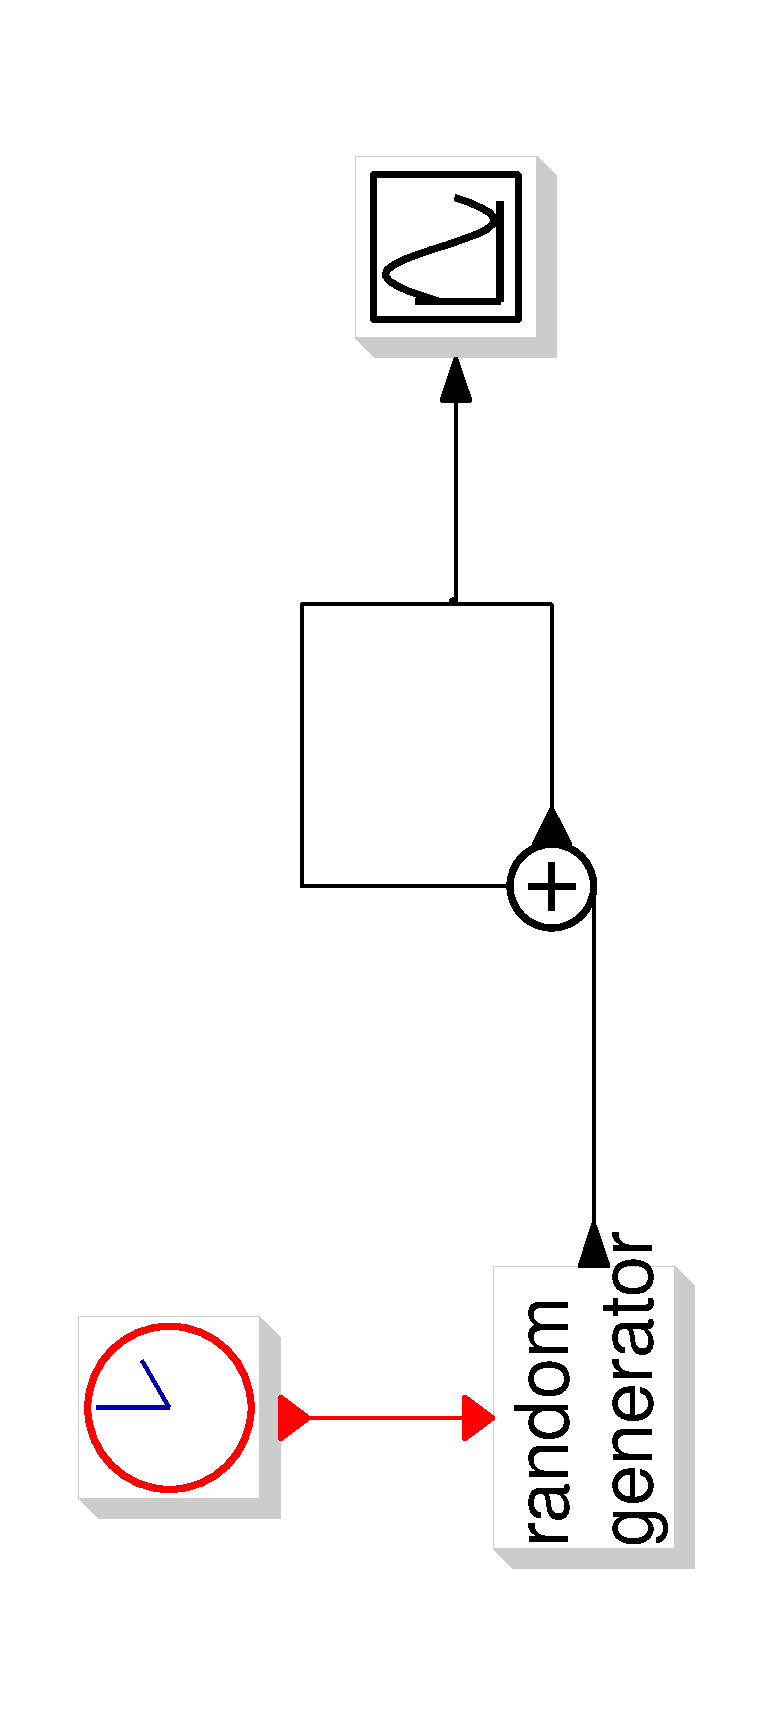
\includegraphics[angle=-90, totalheight=.45\textwidth]{alg_loop.eps}
		\caption{}
		\label{Fig:alg_loop}
	\end{subfigure}
	
	\begin{subfigure}[t]{.5\textwidth}
		\centering
		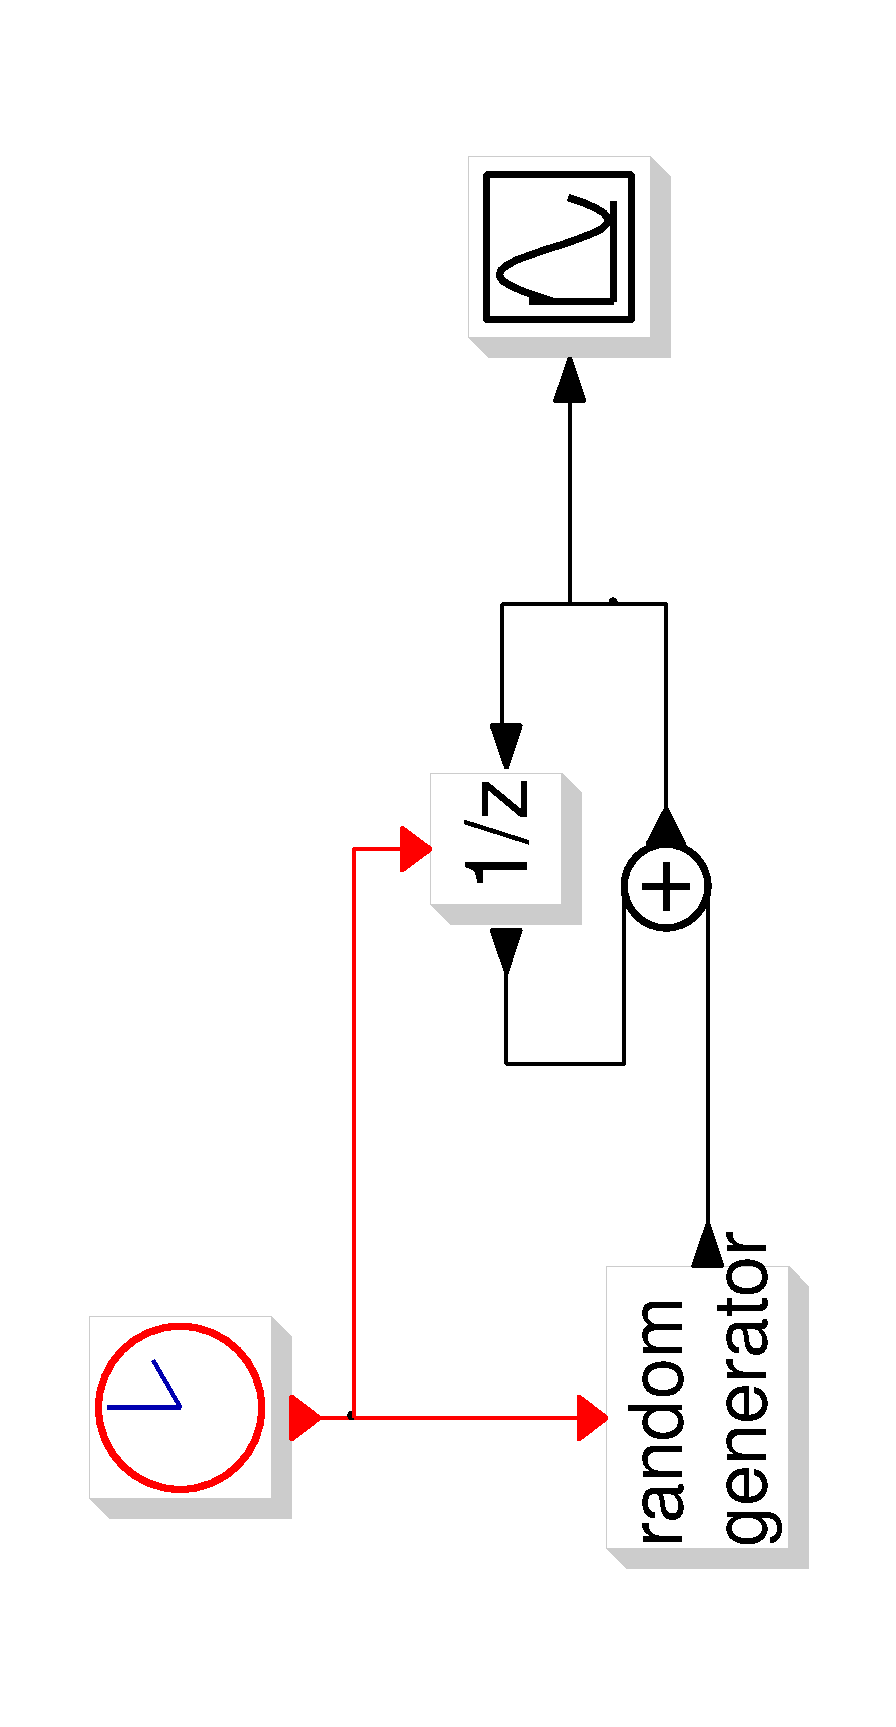
\includegraphics[angle=-90, totalheight=.45\textwidth]{alg_loop_solved.eps}
		\caption{}
		\label{Fig:alg_loop_solved}
	\end{subfigure}
}
\caption{La figura \subref{Fig:alg_loop} mostra un diagramma Scicos che contiene un loop algebrico, mentre in figura \subref{Fig:alg_loop_solved} è raffigurato un diagramma equivalente che risolve il problema inserendo un blocco ritardo.}
\label{Fig:loops}
\end{figure}

%\begin{figure}
%\centering
%\subfloat[\label{Fig:alg_loop}]
%	{\makebox[.5\textwidth][c]{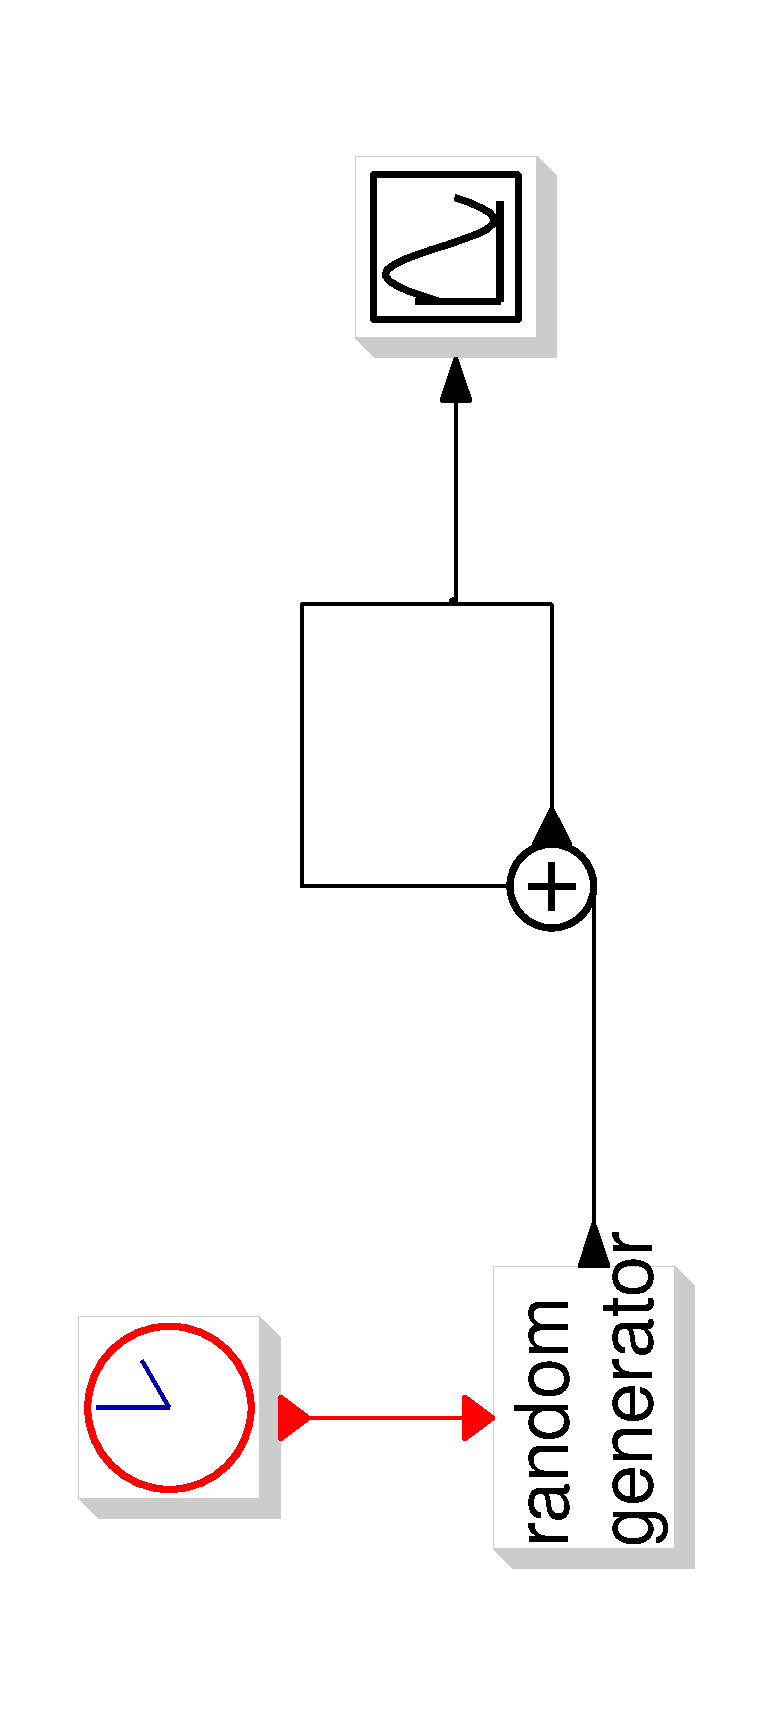
\includegraphics[angle=-90, totalheight=.25\textwidth]{alg_loop.eps}}}
%\subfloat[\label{Fig:alg_loop_solved}]
%	{\makebox[.5\textwidth][c]{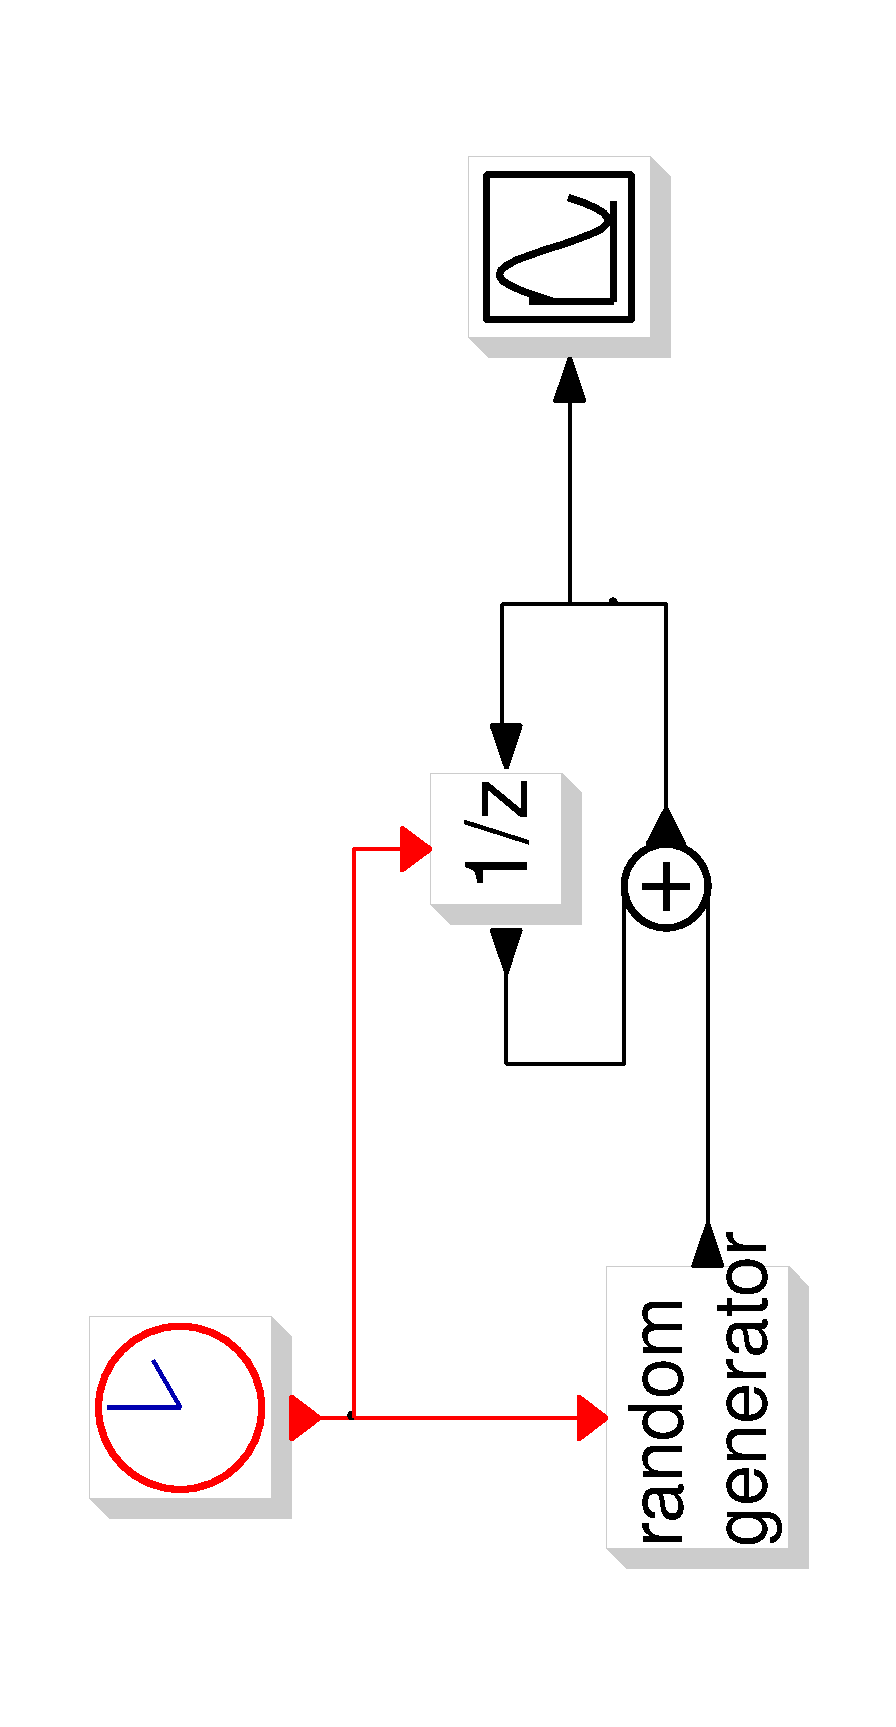
\includegraphics[angle=-90, totalheight=.25\textwidth]{alg_loop_solved.eps}}}
%\caption{La figura \protect\subref{Fig:alg_loop} mostra un diagramma Scicos che contiene un loop algebrico, mentre in figura \protect\subref{Fig:alg_loop_solved} è raffigurato un diagramma equivalente che risolve il problema inserendo un blocco ritardo.}
%\label{Fig:loops}
%\end{figure}